%%%%%%%%%%%%%
% 6-8 Seiten      %
%%%%%%%%%%%%%

\def\verantwortlicher{Gesamte Gruppe} % Dokumentverantwortlicher in Kopfzeile
\thispagestyle{empty} 

%%% Titelseite A
\vspace*{2\baselineskip}

\begin{center}
\sffamily
Universität Leipzig\\
Softwaretechnik-Praktikum\\
Sommersemester 2014
\vskip3\baselineskip

\bgroup
\Huge\textbf{Projektangebot}
\egroup
\vskip3\baselineskip

\begin{tabular}{ll}
Projekt & Graphical SPARQL Builder \\
Gruppe & s14.swp.gsb \\
Verantwortlich & \verantwortlicher\\
Erstellt am & \today \\
\end{tabular}
\end{center}

\vfill%\vskip5\baselineskip

\tableofcontents
%%% Titelseite E

\pagebreak

%%%%%%%%%%%%%%%%%%%%%%%%%%%%%%%%%%%%%%%%
\section{Zielbestimmung}

Eine der wichtigsten Leistungen des World Wide Web ist sicherlich das
Angebot immenser Mengen frei zugänglichen Wissens.
Ein Teil dieses Wissens liegt dabei in einer Vielzahl von Datenbanken,
welche dem Semantic Web zugeordnet sind.
Dieses Konzept steht für die Bereitstellung von Daten auf eine maschinell verarbeitbare Weise, wodurch Suchanfragen, Austausch und Verknüpfungen von Daten, sowie strukturierte Erzeugung und Verwertung von Metadaten möglich werden.
Für die Suche in solchen RDF-basierten Datenbanken stellt SPARQL als
Anfragesprache ein mächtiges Werkzeug dar - für den eingelernten
Nutzer. 
Dieses Projekt verfolgt als Ziel die Entwicklung eines Graphical-SPARQL-Builders
(GSB) und spricht im Vergleich dazu vor allem diejenigen an, denen es
an Erfahrungswerten in Bereichen der SPARQL-Syntax bzw. RDF-Graphen
allgemein mangelt.
Der GSB als graphische Webanwendung soll eine eingängige
Benutzeroberfläche bereitstellen, die eine Vielzahl von Anfragen an
SPARQL-Endpunkte ermöglicht.
Der Schwerpunkt soll dabei vor allem auf einer einfachen, intuitiven Bedienung liegen, welche die darunterliegende SPARQL-Syntax weitestgehend abstrahiert, um ohne aufwendige Einarbeitung die Eingabe komplexer Anfragemuster zu ermöglichen.


%%%%%%%%%%%%%%%%%%%%%%%%%%%%%%%%%%%%%%%%
\section{Voraussetzungen}

Dem GSB geht kein Projekt voraus und er muss somit komplett neu
entwickelt werden.
Technische Voraussetzungen sind die Standardwebtechnologien HTML und
JavaScript, die von einem Webserver ausgeliefert und vom Browser des
Nutzers interpretiert werden.
Der Browser führt hierbei das Programm komplett aus und fragt nur zum Zwecke des Austauschs von Daten den SPARQL-Endpoint via AJAX an. 

\begin{description}
\item[Webserver]
  Für die erfolgreiche Nutzung des Programms muss ein Webserver bereitgestellt   werden, auf dem das Produkt laufen kann und von dem aus online auf den Dienst zugegriffen werden kann.

\item[Datenbanksystem]
  Ein Datenbanksystem wird benötigt, welches die Tripel, die das Produkt verwendet, verwaltet. Beispiele für solche Triplestores sind DBpedia und CPL (catalogus professorum lipsiensis).

\item[Client]
  Der Client selbst benötigt einen Webbrowser zur Ausführung des Programms, bzw. zur Darstellung der Daten. Dieser muss in der Lage sein moderne Sprachen wie HTML5 und JavaScript zu unterstützen. Inbegriffen sind hierbei beliebte Browser wie Firefox, Chrome und Internet Explorer.
\end{description}

%%%%%%%%%%%%%%%%%%%%%%%%%%%%%%%%%%%%%%%%
\section{Designübersicht und Funktionalität}

\subsection{Nutzer Use Cases}

\subsubsection{Benutzer}

Benutzer werden hier als diejenige (Ziel-)Gruppe von Personen definiert, die den GSB verwenden werden, um bestimmte Daten aus einer RDF-Datenbank zu extrahieren.
Benutzer können Anfragen an den vom Administrator bestimmten Endpunkt der RDF-Datenbank mit Hilfe der zur Verfügung gestellten grafischen Oberfläche zusammenstellen und eine Ergebnisausgabe anfordern. Sie können außerdem eine Anleitung einsehen, die ihnen die Nutzung erleichtern soll.

\subsubsection{Administrator}

Der Administrator ist diejenige Person, welche über erweiterte Zugriffsrechte verfügt, die ihm ermöglichen, Funktionalitäten der Anwendung bedarfsmäßig anzupassen.
Dazu zählen hauptsächlich die Anpassung des Endpoints und der Spracheinstellungen. Denkbar sind außerdem Änderungen in der Anfragesyntax, wie etwa das Hinzufügen eines neuen Filters. Dies würde aber über den Rahmen des Projekts hinausgehen.

\subsection{SPARQL Use Cases}
Im Folgenden wird die Struktur von Anfragen im GSB dargestellt und am Beispiel die daraus resultierende SPARQL-Anfrage aufgezeigt.

\subsubsection*{Die Standardstruktur}
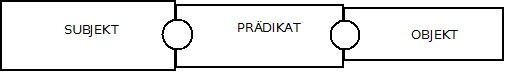
\includegraphics[width=.6\hsize]{01_standard.jpg}


Die Standardstruktur ist dem RDF-Tripel nachempfunden. Das Subjekt entspricht einer Ressource, das Prädikat einem Attribut und das Objekt ist Teil der Menge der Ressourcen und konkreten Werte.

\subsubsection*{Logische Verknüpfungen}
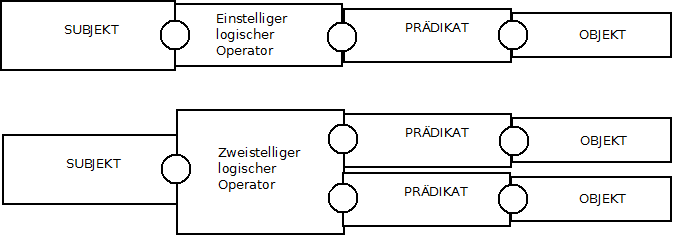
\includegraphics[width=.8\hsize]{02_logVK.jpg}


Logische Operatoren können zwischen Subjekt und Prädikat stehen. Sie werden nach Stelligkeit in zweistellige Operatoren (\verb+AND+, \verb+OR+, \verb+NAND+, \verb+XOR+) und den einstelligen Operator \verb+NOT+ unterteilt.

\subsubsection*{Mengentheoretische Verknüpfungen}
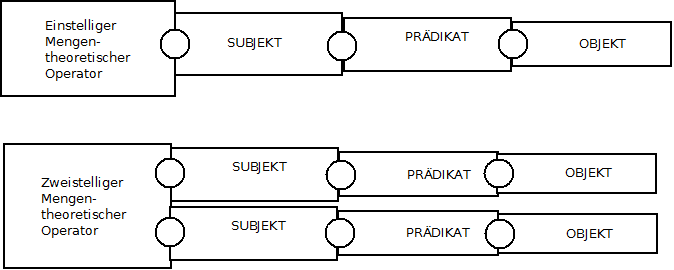
\includegraphics[width=.8\hsize]{03_mengenVK.jpg}

Mengentheoretische Operatoren stehen vor Subjekten. Sie werden wie die logischen Operatoren anhand ihrer Stelligkeit unterschieden: Zweistellige Operatoren (Vereinigung, Schnitt und Differenz) sowie der einstellige Mengenoperator Kardinalität (\verb+COUNT+).

\subsubsection*{Reihungen}
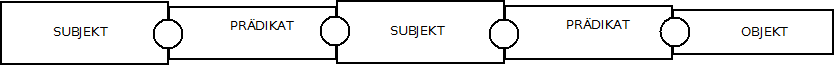
\includegraphics[width=\hsize]{04_reihung.jpg}


Strukturen können “in eine Reihe” gesetzt werden, wenn das Objekt der ersten Struktur das Ergebnis der zweiten Struktur sein soll.

\subsubsection*{Arithmetische Verknüpfung}
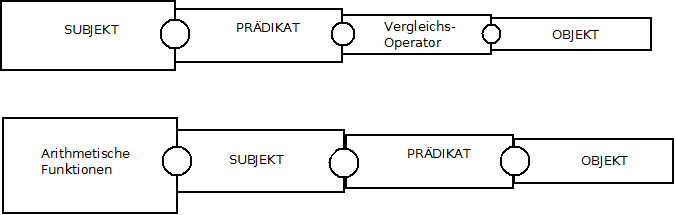
\includegraphics[width=.8\hsize]{05_arithVK.jpg}

Arithmetische Operatoren werden in diesem Kontext unterteilt in Vergleichsoperatoren, welche vor dem Objekt stehen können und arithmetische Funktionen (\verb+MAX+, \verb+MIN+, \verb+AVG+, \verb+SUM+), welche vor dem Subjekt stehen und nur angewandt werden sollten wenn das Ergebnis der folgenden Struktur eine Menge von Zahlen ist.

\subsection*{Beispiele mit den entsprechenden SPARQL-Anfragen}

\subsubsection*{Die Standardstruktur}

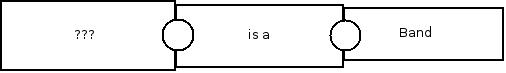
\includegraphics[width=.6\hsize]{bsp01_standard_n.jpg}

\begin{verbatim}
select ?s
where
{
?s a <http://dbpedia.org/ontology/Band>.
}
\end{verbatim}

\subsubsection*{Logische Verknüpfungen}

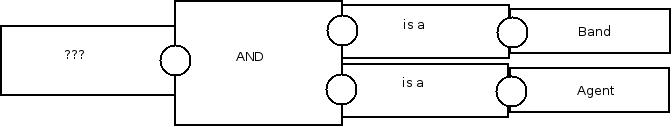
\includegraphics[width=.8\hsize]{bsp02_logVK_n.jpg}

\begin{verbatim}
select ?s
where
{
?s a <http://dbpedia.org/ontology/Band>.
?s a <http://dbpedia.org/ontology/Agent>.
}
\end{verbatim}

\subsubsection*{Mengentheoretische Verknüpfungen}

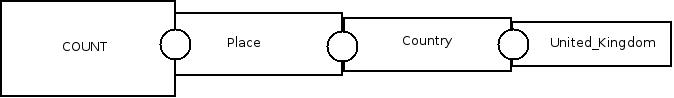
\includegraphics[width=.8\hsize]{bsp03_mengenVK_n.jpg}

{\footnotesize
\begin{verbatim}
select count(*)
where
{
?s a <http://dbpedia.org/ontology/Place>.
?s <http://dbpedia.org/ontology/country> <http://dbpedia.org/resource/United_Kingdom>.
}
\end{verbatim}
}

\pagebreak

\subsubsection*{Reihungen}

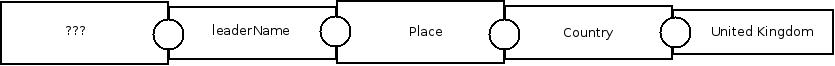
\includegraphics[width=\hsize]{bsp04_reihung_n.jpg}

{\footnotesize
\begin{verbatim}
select ?bm
where
{
?stadt <http://dbpedia.org/ontology/leaderName> ?bm.
?stadt <http://dbpedia.org/ontology/country> <http://dbpedia.org/resource/United_Kingdom>.
}
\end{verbatim}
}

\subsubsection*{Arithmetische Verknüpfung}

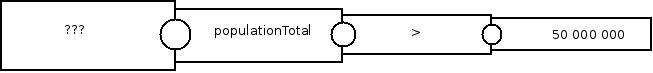
\includegraphics[width=.8\hsize]{bsp05_arithVK_n.jpg}

\begin{verbatim}
select ?s
where
{
?s <http://dbpedia.org/ontology/populationTotal> ?o.
FILTER(?o > 50000000 ).
}
\end{verbatim}




%%%%%%%%%%%%%%%%%%%%%%%%%%%%%%%%%%%%%%%%
\section{Arbeitspakete und Meilensteine}

\subsection{Vorprojekt (30\% des Gesamtprojekt)}

\subsubsection*{Muss-Ziele}

\paragraph{/M1/001} Entwicklung eines graphischen Modells für SPARQL-Anfragen
\paragraph{/M1/002} Beispielhafte Umsetzung ausgewählter SPARQL-Anfragen mit AngularJS

\subsection{Graphische Umsetzung (40\%)}

\subsubsection*{Muss-Ziele}

\paragraph{/M2/001} Umsetzung notwendiger SPARQL-Anfragen

\subsubsection*{Kann-Ziele}

\paragraph{/K2/001} Umsetzung nicht geforderter SPARQL-Anfragen
\paragraph{/K2/002} Modulare Entwicklung um Erweiterbarkeit sicherzustellen
\paragraph{/K3/003} Speichern von Anfragen / Beispielanfragen
\paragraph{/K3/004} i18n

\subsection{Endpoint-Anbindung (20\%)}

\subsubsection*{Muss-Ziele}

\paragraph{/M3/001} Anbindung über Konfigurationsdateien
\paragraph{/M3/002} Beispielhafte Anbindung des GSB an dbpedia Endpoint 

\subsubsection*{Kann-Ziele}

\paragraph{/K3/001} Anbindung an mehrere Endpoints
\paragraph{/K3/002} Caching von Daten um Reaktionszeiten zu verkürzen

\subsection{Benutzerhandbuch (10\%)}

\subsubsection*{Muss-Ziele}

\paragraph{/M4/001} Schriftliches Benutzerhandbuch

\subsubsection*{Kann-Ziele}

\paragraph{/K4/001} Video-Anleitung für Benutzer


%%%%%%%%%%%%%%%%%%%%%%%%%%%%%%%%%%%%%%%%
\section{Qualitätssicherung}

\begin{table}[!h]
  \begin{tabular}{l l l l l}
\toprule
Produktqualität & sehr gut & gut & normal & nicht relevant \\\midrule

Funktionalität & $\times$ \\
Zuverlässigkeit &&& $\times$ \\
Benutzbarkeit &  $\times$ \\
Effizienz  && $\times$ \\
Anpassbarkeit &&& $\times$ \\
Übertragbarkeit &&& $\times$ \\
\bottomrule
\end{tabular}
\end{table}

Erläuterungen:
Da der GSB als eingängige, benutzerfreundliche Webapplikation ausgelegt ist, stehen Benutzbarkeit und Funktionalität klar im Vordergrund, da diese Aspekte als Kernargumente für die Nutzung der Anwendung klare Priorität haben.
Zuverlässigkeit spielt eine weniger entscheidende Rolle. Abstürze sind natürlich nie erwünscht, doch müssen hier etwa keine wichtigen Daten vor einem Verlust bewahrt werden, oder Nutzertransaktionen mit allen Mitteln abgesichert werden.
Effizienz ist definitiv wichtig, wenn es um Operationen auf Datenbanken geht. Da in den meisten Fällen mit großen Mengen von Daten gearbeitet wird, und die Datenanfrage die zentrale Aufgabe des GSB darstellt, ist es wünschenswert, dass die Anwendung diese in zufriedenstellender Zeit bearbeiten und Ergebnisse präsentieren kann.
Anpassbarkeit könnte besonders im Bezug auf die Sprache der Anwendungsoberfläche und eine Erweiterung der Anfragemöglichkeiten von Interesse sein. Doch da dieses Projekt sich mehr als 'Grundsteinlegung' einer graphischen SPARQL-Anfragehilfe versteht, werden sich auch die Ressourcen zunächst entsprechend anderweitig konzentrieren.
Übertragbarkeit bezieht sich im Falle des GSB  hauptsächlich auf die Möglichkeit, Anfragen an unterschiedliche Endpunkte zu stellen, bis hin zu einer kombinierten Anfrage auf mehrere Endpoints. Da Ersteres zunächst nur über eine Konfigurationsdatei abgehandelt wird, und Letzteres in seiner Komplexität den Rahmen dieses Projekts sprengen würde, wird diesem Aspekt ebenfalls eine abgeschwächte Priorität zugeordnet.


%%%%%%%%%%%%%%%%%%%%%%%%%%%%%%%%%%%%%%%%
\section{Glossar}
% SIGGI: ANMERKUNG: Bitte aus Recherchebericht übernehmen und nicht benötigte Sachen wie URI oder was weiß ich löschen und folgenden hinzufügen -- Lukas

% SIGGI: Ok mach ich, wenn noch jemand wünsche für den Glossar hat schreibt die hier hin.
% Je nach lust und laune morgen und je nachdem wie lang das ganze wird werd ich eventuell das ein oder andere aus eueren texten in den glossar übernehmen.
% ToDo an mich selbst: Korrekturen am letzten Glossar vorhnehmen

\newcommand{\begriff}[2]{
\paragraph{#1}
#2
}

%\begin{itemize}

\begriff{API}
{Application Programming Interface -- Programmierschnittstelle.
Eine API be\hack{-\break}schreibt, wie Software-Komponenten bzw. Programme miteinander interagieren können/sollten. Anders ausgedrückt: eine API ist der Teil eines Softwaresystems, der anderen Programmen zur Verfügung gestellt wird um mit dem Softwaresystem zu interagieren.}

\begriff{DBpedia}
{DBpedia ist eine Datensammlung im RDF Format, deren Datensätze aus der Wikipedia extrahiert wurden. Ziel ist es strukturierte Daten für Webanwendungen zur Verfügung zu stellen.
\cite{dbpedia-wikipedia,dbpedia,dbpedia-datasets}
}

\begriff{Endpoint}
{Ein Endpoint ist eine Schnittstelle zwischen der Datensammlung und der 
Abfragesprache. Nachdem eine Anfrage an den Endpoint gesendet wurde (query)  sendet selbiger die Ergebnisse zurück. Ein Beispiel für einen SPARQL-Endpoint ist der “Virtuoso SPARQL Query Editor”. \cite{dbpedia-sparql}}

\begriff{GSB}
{Graphical SPARQL Builder, der Name des Projekts. \cite{swp14-gsb}}

\begriff{i18n} internationalization and localization -- Anpassung der Software an andere Sprachen und Kulturen ohne Quelltext zu ändern. Sprach- und Kulturspezifika werden über Konfigurationsdateien angepasst. 

% \begriff{IRI}
% {“Internationalized Resource Identifier” kurz IRI ist eine spezialisierte Form der URI, die
%  nur ASCII-Zeichen enthält. \cite{iri,rfc3987}}

% \begriff{JSON}
% {Javascript Object Notation -- eine Dateiformat für den Datenaustausch zwischen Anwendungen. JSON soll für Mensch und Maschine gleichermaßen einfach lesbar sein und sich durch Kompaktheit auszeichnen. Dabei soll jedes gültige JSON Dokument gültiges Javascript darstellen.
% \cite{json}
% }

\begriff{Ontologie}
{Ontologien sind formalisierte Vokabulare von Begriffen. Diese Vokabulare beziehen sich meist auf eine bestimmte Domäne (Gegenstandsbereich) oder Nutzergruppe. Sie liegen in einer sprachlichen Form vor und umfassen die Begriffe einer Domäne sowie Beziehungen zwischen den Begriffen. \cite{owl,ontologie-wiki,fraunhofer}
}

\begriff{OWL}
{Die Web Ontology Language (OWL, aktuelle Version OWL2) ist eine Beschreibungssprache um Ontologien für das semantische Web zu erstellen und zu publizieren. OWL2-Ontologien können für Informationen verwendet werden, die in RDF geschrieben sind und werden hauptsächlich in Form von RDF-Dokumenten ausgetauscht.
\cite{owl}
}

\begriff{RDF}
{“Resource Description Framework” kurz RDF ist eine Strukturierung von Daten nach
dem Muster Subjekt-Prädikat-Objekt. Alle RDF-Daten werden in diesem Tripel-Format 
gespeichert. RDF gilt als eines der Basis-Elemente des semantischen Webs.
Repräsentationen, also syntaktische Standards, des RDF-Prinzips sind N3 (Notation3), 
Turtle (Terse RDF Triple Language) sowie RDF/XML. Turtle und N3 gelten im Vergleich zu RDF/XML als benutzerfreundlicher. \cite{rdf-primer,rdf-wiki,rdf-xml-wiki}}

% \begriff{RDF-Modelle als gerichtete Graphen}
% {Aussagen werden in RDF als Tripel modelliert. Eine Menge solcher Tripel bildet einen gerichteten Graph, wobei Subjekte Objekte die Knoten und Prädikate die Kanten darstellen. \cite{rdf-wiki}}

% \begriff{RDFS}
% {“Resource Description Framework Schema” kurz RDFS ist ein Konzept für den 
% Austausch von Daten. Durch Syntax-Vorgaben wird eine einheitliche und umfassendere
% Interpretation der Daten ermöglicht. \cite{w3c-rdf-schema}}

% \begriff{Reasoning}
% {Als Reasoning bezeichnet man ein Ableitungsverfahren mit dem aus RDF-Daten durch gegebene Regeln und Strukturen neue Daten beziehungsweise deren Verknüpfung erzeugt werden können. \cite{reasoning-paper,rdf-reasoning}}

\begriff{SPARQL}
{“SPARQL Protocol And RDF Query Language” kurz SPARQL ist eine Abfragesprache für das Datenformat RDF. SPARQL ist graphbasiert und gilt nach dem W3C als Standard für RDF-Abfragen. \cite{w3c-rdf-sparql-query,sparql-wiki}}

\begriff{Triplestore}
{Ein Triplestore ist ein System zur Speicherung, Verwaltung und Bearbeitung einer
 Sammlung von RDF-Tripeln. Ein Triplestore bietet gewöhnlich APIs,
 Rea\-so\-ning-Verfahren sowie Abfragemöglichkeiten. \cite{fraunhofer}}

% \begriff{URI}
% {“Uniform Resource Identifier” kurz URI sind Ressourcen-Identifikatoren. Sie bestehen 
% aus Schema, Anbieter, Pfad, Abfrage und Teil, wobei nur Schema und Pfad zwingend 
% vorhanden sein müssen. Ein RDF-Objekt wird durch eine URI eindeutig identifiziert. \cite{uri}}

% \begriff{XML}
% {Die Extensible Markup Language (XML) ist eine Auszeichnungssprache. Sie dient der Darstellung hierarchisch strukturierter Daten in Form von Textdateien. Oberstes Design-Ziel ist dabei die Verwendbarkeit zum Datenaustausch über Netzwerke, speziell das Internet. Weiterhin stehen Implementierungs- und Plattformunabhängigkeit sowie Lesbarkeit für Menschen im Vordergrund.
% \cite{xml}
% }



%%%%%%%%%%%%%%%%%%%%%%%%%%%%%%%%%%%%%%%%
\begin{thebibliography}{99}
\bibitem{dbpedia-wikipedia}
  \url{http://de.wikipedia.org/wiki/DBpedia}

\bibitem{dbpedia}
  \url{http://de.dbpedia.org/}

\bibitem{dbpedia-datasets}
  \url{http://wiki.dbpedia.org/Datasets}

\bibitem{dbpedia-sparql}
  \url{http://dbpedia.org/sparql}

\bibitem{swp14-gsb} %5
  \url{http://pcai042.informatik.uni-leipzig.de/~swp14-gsb/}

% \bibitem{iri}
% \url{http://de.wikipedia.org/wiki/Internationalized_Resource_Identifier}

% \bibitem{rfc3987}
% \url{http://tools.ietf.org/html/rfc3987}

% \bibitem{json}
% \url{http://www.json.org}

\bibitem{owl}
  \url{http://www.w3.org/TR/2012/REC-owl2-overview-20121211/}

\bibitem{ontologie-wiki} %10
  \url{http://de.wikipedia.org/wiki/Ontologie}

\bibitem{fraunhofer}
  \url{http://www.iais.fraunhofer.de/fileadmin/user_upload/Abteilungen/OK/PDFs/Alieva_Magisterarbeit.pdf}

\bibitem{rdf-primer}
  \url{http://www.w3.org/TR/rdf-primer/}

\bibitem{rdf-wiki}
  \url{http://de.wikipedia.org/wiki/Resource_Description_Framework}

\bibitem{rdf-xml-wiki}
  \url{https://en.wikipedia.org/wiki/RDF/XML}

% \bibitem{w3c-rdf-schema}
% \url{http://www.w3.org/TR/rdf-schema/}

% \bibitem{reasoning-paper}
% \url{http://www.w3.org/2004/12/rules-ws/paper/47/}

% \bibitem{rdf-reasoning}
% \url{http://elite.polito.it/files/courses/01LHV/2012/4-RDFreasoning.pdf}


\bibitem{w3c-rdf-sparql-query}
  \url{http://www.w3.org/TR/rdf-sparql-query/}

\bibitem{sparql-wiki}
  \url{http://en.wikipedia.org/wiki/SPARQL}

% \bibitem{uri}
% \url{http://de.wikipedia.org/wiki/Uniform_Resource_Identifier}



% \bibitem{xml}
% \url{http://www.w3.org/TR/xml/}

\end{thebibliography}







%%% Local Variables: 
%%% mode: latex
%%% TeX-master: "main"
%%% End: 
